\section{Generovanie HDR}
\label{sec:Theory-Generating}

V úvode vysvetlíme význam premenných, ktoré budú použité nielen pri zápise rovníc, ale aj v zdrojovom
kóde aplikácie:
\begin{itemize}
    \item $P$ - počet obrázkov s rozličnou expozíciou,
    \item $N$ - počet pixelov v jednom obrázku,
    \item $Z_{ij}$ - hodnota pixelu, kde $i$ je index pixelu a $j$ index obrázku,
    \item $Z_{min}$, $Z_{max}$ - hodnota minima a maxima, ktorú môže pixel nadobudnúť,
    \item $\Delta t_{j}$ - expozičný čas pre $Z_{ij}$,
    \item $w(Z_{ij})$ - váhová funkcia odstraňujúca presahujúce hodnoty.
\end{itemize}

Ak by mal fotoaprát lineárnu odozvu, intenzita žiarenia $E$ pre pixel na indexe $i$ by mohla byť 
vytvorená kombináciou hodnôt, zaznamenaných pre každú expozíciu a pre každý farebný kanál ako
\begin{equation}
    E_{i} = \frac{
            \sum_{j=1}^{P}
            \frac{1}{\Delta t_{j}}
            w(Z_{ij})Z_{ij}
        }{
            \sum_{j=1}^{P}
            w(Z_{ij})
        }
    \cite{AHDR}
\end{equation}

Avšak digitálne fotoaparáty nemajú lineárnu odozvu, ale všeobecnú funkciu nazývanú krivka odozvy
fotoaparátu (CRF\footnote{Camera Response Function}). Predtým, ako sa bude generovať HDR obsah,
je potrebné vyjadriť túto krivku odozvy. Na to slúži algoritmus od Paul E. Debeveca a Jitendra Malika, 
založený na využívaní fyzikálnej vlastnosti zobrazovacích systémov, ktorú nazveme reciprocita.
Reciprocita vyjadruje reakciu svetlocitlivého materiálu ako inverzný vzťah medzi intenzitou svetla 
a času osvetlenia. Pri štandardnom rozsahu expozície je odozva fotoaparátu určená celkovou expozíciou 
definovanou ako intenzita $\times$ čas. \cite{AHDR}

\subsection{Získanie krivky odozvy fotoaparátu} 

Vstupom algoritmu sú fotografie vytvorené s rôznou dĺžkou času expozície $\Delta t_{j}$. Za predpokladu, 
že hodnoty intenzity žiarenia $E_{i}$ pre každý pixel $i$ sú konštanty, môžeme zapísať rovnicu 
reciprocity ako:
\begin{equation} \label{eq:reciprocity}
    Z_{ij} = f(E_{i} \Delta t_{j})
    \cite{Debevec}
\end{equation}
Keďže je funkcia $f$ monotónna, potom je aj invertovateľná a rovnicu \ref{eq:reciprocity} môžeme
zapísať ako $f^{-1}(Z_{ij}) = E_{i} \Delta t_{j}$. Pridaním prirodzeného logaritmu na obe strany 
získame \\$\ln f^{-1}(Z_{ij}) = \ln E_{i} + \ln \Delta t_{j}$. Následne si definujeme funkciu
$g = \ln f^{-1}$ a dostaneme súbor rovníc:
\begin{equation} \label{eq:gFunction}
    g(Z_{ij}) = \ln E_{i} + \ln \Delta t_{j}
    \cite{Debevec}
\end{equation}

Cieľom algoritmu je pomocou metódy najmenších štvorcov vyjadriť funkciu krivky odozvy $g$ a intenzitu
žiarenia $E_{i}$, ktoré najlepšie vyhovujú súboru rovníc \ref{eq:gFunction}. Keďže rozsah hodnôt jasu
je konečný, vyjadrujeme iba konečný počet hodnôt krivky odozvy $g$. Vyjadrením celočíselných hodnôt
pixelov $Z_{min}$ a $Z_{max}$, počtu polôh pixelu $N$ a počtu fotografií $P$, definujeme problém ako
hľadanie $(Z_{max} - Z_{min})$ hodnôt pre $g(Z)$ a $N$ hodnôt pre $\ln E_{i}$, ktoré minimalizujú
kvadratickú objektívnu funkciu:
\begin{equation} \label{eq:objFunction}
    \mathcal{O} = 
    \sum_{i=1}^{N}
    \sum_{j=1}^{P}
    [g(Z_{ij}) - \ln E_{i} - \ln \Delta t_{j}]^{2}
    + \lambda
    \sum_{z=Z_{min} + 1}^{Z_{max} - 1}
    g''(z)^{2}
    \cite{Debevec}
\end{equation}
Prvý term zabezpečuje, že riešenie vyhovuje súboru rovníc vyplývajúcich z rovnice \ref{eq:gFunction}
a~druhý term zabezpečuje plynulosť funkcie $g$. Hodnota $\lambda$ je váha plynulosti, relatívna 
k~prvému termu a je zvolená podľa množstva šumu očakávaného v $Z_{ij}$.

\begin{figure}[t]
    \centering
    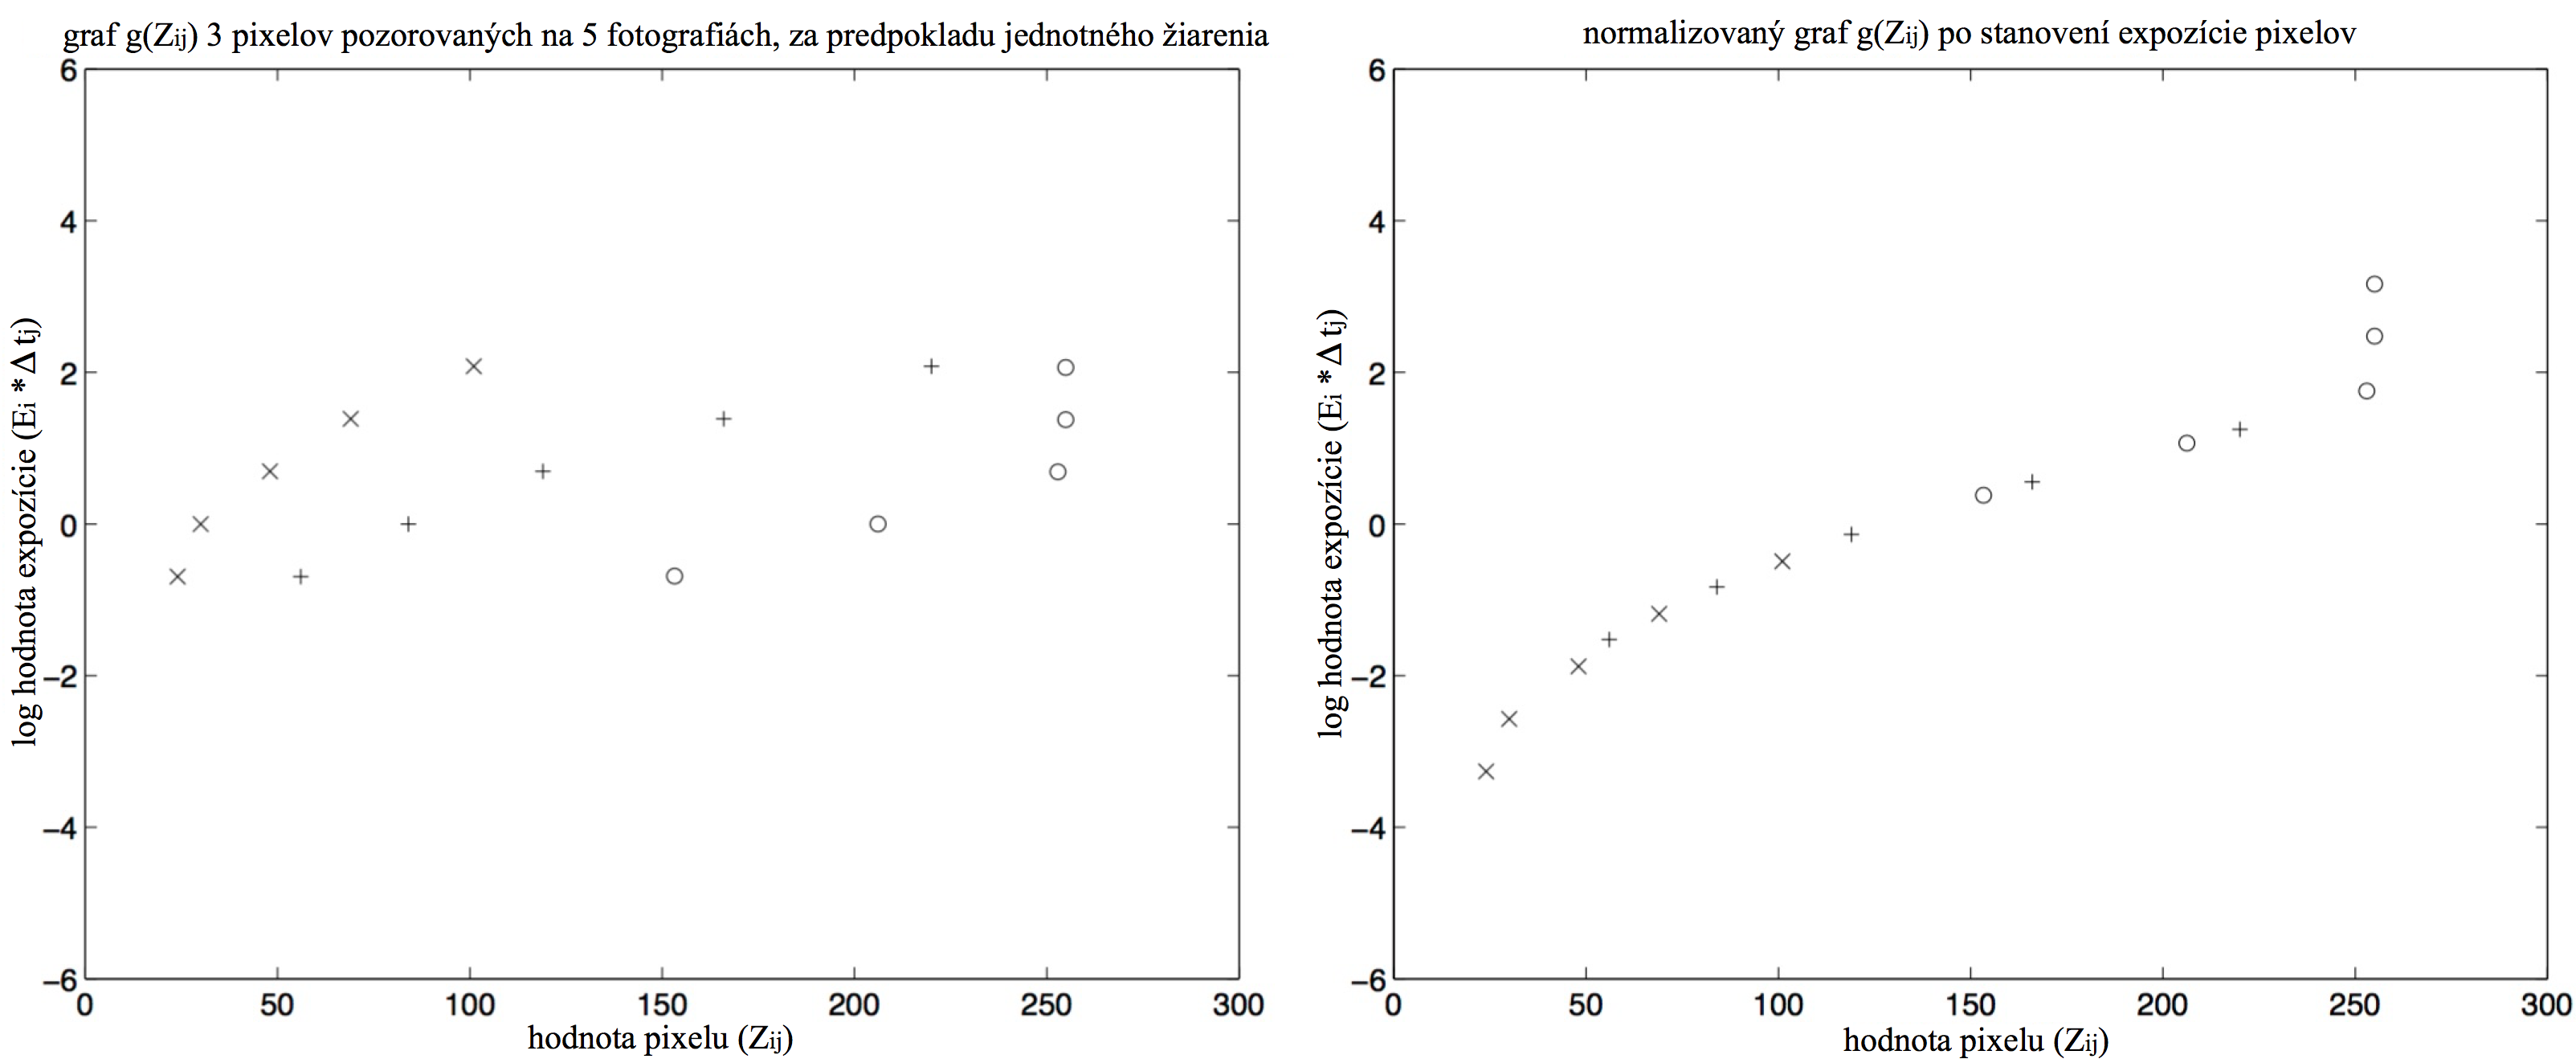
\includegraphics[width=\textwidth]{figures/generating/normalized-curve}
    \caption{Normalizácia hodnôt $Z_{ij}$ riešením rovnice \ref{eq:objFunction} \cite{Debevec}}
\end{figure}
